% todo: colocar script de tratamento dos dados de ITC, pra determinar a cmc
% todo: colocar uma tabela com correlações de concentração (m/m, v/v, mol/l, mol/mol)
\begin{apendicesenv}
\partapendices

\chapter{Descrição matemática do modelo de micelas gigantes}
\label{sec:modelo_MG_matematica}
\section{Introdução e motivação}

% TODO: colocar as referências.
Esta seção mostrará as equações utilizadas para descrever o modelo de espalhamento de micelas gigantes. As equação foram baseadas numa série de artigos de X, Y, Z. Aqui, esses artigos serão agrupados, de modo a facilitar o entendimento do modelo.

Porém, essa descrição matemática é de menor aplicabilidade, pois é necessário transcrever as equações em código que consiga realizar ajustes. Essa tarefa não é trivial, especialmente para não especialistas. Logo, será disponibilizado, na seção X, uma transcrição dessas equações, na linguagem Python.

% TODO: colocar a seção onde o modelo foi utilizado
% TODO: colocar a seção onde a descrição de Python foi escrita
% TODO: reescrever essas equações, colocando os termos qe são texto em \text e o resto normal

\section{Resumo do modelo}

O modelo descreve cadeias alongadas caroço-casca (\emph{core-shell}) de Kratky-Porod, considerando volume excluído, com interações intercadeias modeladas pelo modelo PRISM (\emph{Polymer Reference Interaction Site Model}). No total, a equação de intensidade de espalhamento \(I\) em função do vetor de espalhamento \q (\(I(q)\), Eq. \ref{eqn:AP_saxs_MG_superficial}) possui 13 parâmetros, descritos na tabela \ref{tab_ap:simbolos}.

\begin{equation}
I = f(q, scale, d_{head}, r_{core}, \rho_{rel}, \sigma, back, L, k_L, \varepsilon, D_{CQ}, \nu_{RPA}, SC_{pow}, exp_{pow})
\label{eqn:AP_saxs_MG_superficial}
\end{equation}
% TODO: colocar refs às equações que definem alguns desses termos
\begin{table}
    \IBGEtab%
    {\caption{Símbolos e parâmetros utilizados no modelo, e seus significados}
     \label{tab_ap:simbolos} }%
    {\begin{tabular}{r p{8cm}}
    	\toprule
     Símbolo 			& Descrição        						\\
     \midrule
     \(I\)					& Intensidade de RX espalhado			\\
     \q					& Vetor de espalhamento					\\
     \midrule
     \(scale\)				& Fator de escala						\\
     \(d_{head}\)			& Espessura do \emph{shell}				\\
     \(r_{core}\)			& Raio do \emph{core}					\\
     \(\rho_{rel}\)		& Diferença de densidade eletrônica entre \emph{core} e \emph{shell} \\
     \(\sigma\)			& Fator de \emph{smearing}, o quão definido é o limite entre regiões \\
     \(back\)				& Constante referente ao \emph{background} \\
     \(L\)					& Comprimento de contorno das cadeias 	\\
     \(k_L\)				& Comprimento de \emph{Kuhn} das cadeias, igual ao dobro do comprimento de correlação \\ % TODO: Achar o que é esse comprimento exatamente
     \(\varepsilon\)			& Excentricidade radial das micelas		\\
     \(D_{CQ}\)			& Distância de correlação das micelas 	\\
     \(\nu_{RPA}\)			& Fator de concentração					\\
     \midrule
     \(SC_{pow}\)			& Fator de escala (pre-exponencial) da exponencial em baixo q\\
     \(exp_{pow}\)			& Fator exponencial, relativo à inclinação na escala log\\
     \bottomrule
    \end{tabular}}%
    {}%
\end{table}

A equação geral do modelo, e a descrição de seus fatores, estão descritos na Eq.\ref{eqn:AP_saxs_MG_geral} e na Tab. \ref{tab_ap:fatores_geral}.

\begin{equation}
I = \frac{scale\left(F_{KPchain_{ExV}}F_{rod_{CS}}\right)}{1 + \nu_{RPA} F_{sphere}\left( D_{CQ}\right) F_{KPchain_{ExV}}} + back + scale_{pow}^{-exp_{pow}}
\label{eqn:AP_saxs_MG_geral}
\end{equation}

\begin{table}
    \IBGEtab%
    {\caption{Parâmetros da equação \ref{eqn:AP_saxs_MG_geral}}
     \label{tab_ap:fatores_geral} }%
    {\begin{tabular}{r p{8cm}}
    \toprule
    Termo 			& Descrição        						\\
    \midrule
    \(F_{KPchain_{ExV}}\)  & Fator forma de cadeias de Kratky-Porod com volume excluído \\
    \(F_{rod_{CS}}\)		 & Fator forma da seção transversão de um bastão	\\
    \(F_{sphere}(D_{CQ})\) & Fator forma de uma esfera, cujo raio é a distância de correlação \\
    \bottomrule%
    \end{tabular}}
    {}%
\end{table}


Já o modelo do PRISM é descrito pela Eq. \ref{eqn:AP_saxs_PRISM}. Note a similaridade com a Eq \ref{eqn:AP_saxs_MG_geral}.

\begin{equation}
I_{PRISM}= \frac{\varphi V_{mic}F_{wc}(q)F_{cs}(q)}{1 + \nu F_{rod}(qL_{c(q)})F_{wc}(q)}
\label{eqn:AP_saxs_PRISM}
\end{equation}

\begin{table}
    \IBGEtab{%
      	\caption{Termos da equação \ref{eqn:AP_saxs_PRISM}}
    \label{tab_ap:PRISM_geral}}%
    {%
     \begin{tabular}{r p{8cm}}
     \toprule
     Termo 			& Descrição        						\\
     \midrule
     \(\varphi\)		& Fração volumétrica \\ % TODO: checar
     \(V_{mic}\)		& Volume da micela   \\
     \(F_{wc}\)		& Fator forma de uma \emph{wormlike chain} \\
     \(F_{cs}\)		& Fator forma de uma seção transversal de cilindro \\ % TODO: checar se é cilindro
     \(F_{rod}\)		& Fator forma de um bastão infinitamente longo \\
     \(L_{c(q)}\)		& \(=6\xi\), comprimento característico \\
     \(\xi\)			& Comprimento de correlação da função \(c(q) \approx F_{rod}\) \\
     \bottomrule
     \end{tabular}}%
     {}%
\end{table}


A partir disso, podemos começar a adentrar nos termos.

\section{Descrição detalhada do modelo}

O modelo será dividido em duas partes, uma referente à cadeia micelar, \(F_{wc}\) e outra referente à seção transversal da cadeia, \(F_{cs}\).

\subsection{Fator forma das cadeias \emph{wormlike}, \(F_{wc}\)}
\label{sec:equacoes_Fwc}

\begin{equation}
F_{wc} = \left[\left(1 - \chi\right)F_{chain_{ExV}} + \chi F_{rod}\right]\Gamma
\label{eqn:AP_Fwc}
\end{equation}

% TODO: colocar a equação do \Gamma
A equação \ref{eqn:AP_Fwc} pode ser simplificada dependendo da faixa de \q. A região de \q intermediária precisa ser descrita pelo termo \(\chi\) (Eq. \ref{eqn:AP_chi}) e corrigida por \(\Gamma\). Esses parâmetros são obtidos por simulações de Monte Carlo.

\begin{equation}
	F_{\text{wc}} \approx 
		\begin{cases}
			F_{\text{chain}_{\text{ExV}}}		& \text{q baixo}  \\
			F_{\text{rod}}						& \text{q alto}
		\end{cases}
	\label{eqn:AP_Fwc_dois_casos}
\end{equation}

%	\begin{longtable}[c]{r p{12cm}}
%		\toprule
%		Termo 			& Descrição        						\\
%		\midrule
%		\(\chi\)			& Região de \emph{crossover} \\
%		\(\Gamma\)		& Correção da região de crossover. \\
%		\bottomrule
%		\caption{Termos da equação \ref{eqn:AP_Fwc}}
%		\label{tab_ap:Fwc} 
%	\end{longtable}

\subsubsection{Fator de correção \(\chi\)}
O termo \(\chi\) é descrito pela equação \ref{eqn:AP_chi}, que por sua vez é dependente da equação \ref{eqn:AP_xi}.

\begin{equation}
\chi = \exp{\xi^{-5}}
\label{eqn:AP_chi}
\end{equation}

% todo: achar o significado do termo b
\begin{equation}
\xi = q k_L\left(\frac{\pi b}{1,103L}\right)^{3/2}\left(\frac{\left<R_g^2\right>}{k_L^2}\right)^{1,282}
\label{eqn:AP_xi}
\end{equation}

\noindent onde \(\left<R_g^2\right>\) é a média do \emph{ensemble} do quadrado do raio de giro das cadeias, no modelo.

\subsubsection{Fator forma de cadeias com volume excluído, \(F_{chain_{ExV}}\)}
\label{sec:F_chain_ExV_equacoes}
O termo \(F_{chain_{ExV}}\) possui a seguinte forma (Eq. \ref{eqn:AP_FchainExV})

% TODO: verificar se o \nu aqui é o \nu_RPA
\begin{multline}
F_{chain_{ExV}} = w(qR_g)F_{Debye}(q,L,k_L) + \left[1 - w(q R_g)\right] \\ \left[C_1(q R_g)^{\frac{1}{\nu}} + C_2(q R_g)^{-\frac{2}{\nu}} + 
C_3(q R_g)^{-\frac{3}{\nu}}\right]
\label{eqn:AP_FchainExV}
\end{multline}
% todo: colocar o valor de \nu, que está na Eq. S_EXV_APP
% todo: incluir aqui uma tabela com os termos e as equações

O termo \(F_{Debye}\), por sua vez, é dado pela Eq. \ref{eqn:AP_fdebye}.
\begin{equation}
F_{Debye} = 2 \left(\frac{e^{-u} + u - 1}{u^2}\right)
\label{eqn:AP_fdebye}
\end{equation}

\noindent onde \(u = R_g^2q^2\). \(R_g\) é a raiz quadrada do raio de giro médio ao quadrado, \(R_g = \left<R_g^2\right>^{1/2}\), considerando o volume excluído. Por sua vez, esse valor é dado pela Eq. \ref{eqn:AP_Rg2}

% todo: Achar o que significam os termos faltantes aqui.
\begin{equation}
\left<R_g^2\right> = \alpha \left(\frac{L}{k_L}\right)^2\left<R_g^2\right>_0
\label{eqn:AP_Rg2}
\end{equation}

O termo \(w\) é uma equação empírica, da forma: (Eq \ref{eqn:AP_w})

\begin{equation}
w(x) = \frac{\left[1 + \frac{\tanh(x-C_4)}{C_5}\right]}{2}
\label{eqn:AP_w}
\end{equation}

As constantes \(C_1\), \(C_2\), \(C_3\), \(C_4\) e \(C_5\) foram obtidas a partir de um ajuste, e estão na tabela \ref{tab_ap:C1C5}, assim como o valor de \(\nu\).
\begin{table}
    \IBGEtab%
    {\caption{Constantes}
    \label{tab_ap:C1C5} }%
    {\begin{tabular}{r p{2cm}}
      \toprule
      Constante 	& Valor \\
      \midrule
      \(C_1\)			&  1,220	\\
      \(C_2\)			&  0,4288	\\
      \(C_3\)			&  -1,651	\\
      \(C_4\)			&  1,523	\\
      \(C_5\)			&  0,1477 	\\	
      \(\nu\)			&  0,585	\\					
      \bottomrule
    \end{tabular}}% todo: encontrar de onde vem o \nu
    {}%
\end{table}


\subsubsection{Fator de correção \(\Gamma\)}

O fator de correção \(\Gamma\) (Eq. \ref{eqn:AP_Gamma}) é dependente de dois conjuntos de constantes, \(A\) (Eq. \ref{eqn:AP_Ai}) e B (Eq. \ref{eqn:AP_Bi}) determinadas empiricamente (Tab \ref{tab_ap:AiBi}).

\begin{equation}
\Gamma\left( q,L,k_{L} \right) = 1 + \left( 1 - \chi \right)\sum_{i = 2}^{5}{A_{i}\xi^{i}} + \chi\sum_{i = 0}^{2}{B_{i}\xi^{- i}}
\label{eqn:AP_Gamma}
\end{equation}

\begin{equation}
A_{i} = \sum_{j = 0}^{2}{a_{1}\left( i,j \right)\left( \frac{L}{k_{L}} \right)^{- j}\exp\left( - \frac{10k_{L}}{L} \right)} + \sum_{j = 1}^{2}{a_{2}\left( i,j \right)\left( \frac{L}{k_{L}} \right)^{j}\exp\left( - \frac{2L}{k_{L}} \right)}
\label{eqn:AP_Ai}
\end{equation}

\begin{equation}
B_{i} = \sum_{j = 0}^{2}{b_{1}\left( i,j \right)\left( \frac{L}{k_{L}} \right)^{- j}\ } + \sum_{j = 1}^{2}{b_{2}\left( i,j \right)\left( \frac{L}{k_{L}} \right)^{j}\exp\left( - \frac{2L}{k_{L}} \right)}
\label{eqn:AP_Bi}
\end{equation}

\begin{table}[h]
    \IBGEtab%
    {\caption{Constantes utilizadas para o cálculo de \(\Gamma\)}
    \label{tab_ap:AiBi}}%
    {\begin{tabular}{r l | r l | r l | r l}
    	\toprule
    	\(a_1\)(2,0) & --0.1222 & \(a_2\)(2,1) & 0.1212   & \(b_1\)(0,0) & --0.0699 & \(b_2\)(0,1) & --0.5171 \\
    	\(a_1\)(3,0) & 0.3051   & \(a_2\)(3,1) & --0.4169 & \(b_1\)(1,0) & --0.09   & \(b_2\)(1,1) & --0.2028 \\
    	\(a_1\)(4,0) & --0.0711 & \(a_2\)(4,1) & 0.1988   & \(b_1\)(2,0) & 0.2677   & \(b_2\)(2,1) & --0.3112 \\
    	\(a_1\)(5,0) & 0.0584   & \(a_2\)(5,1) & 0.3435   & \(b_1\)(0,1) & 0.1342   & \(b_2\)(0,2) & 0.6950   \\
    	\(a_1\)(2,1) & 1.761    & \(a_2\)(2,2) & 0.0170   & \(b_1\)(1,1) & 0.0138   & \(b_2\)(1,2) & --0.3238 \\
    	\(a_1\)(3,1) & 2.252    & \(a_2\)(3,2) & --0.4731 & \(b_1\)(2,1) & 0.1898   & \(b_2\)(2,2) & --0.5403 \\
    	\(a_1\)(4,1) & --1.291  & \(a_2\)(4,2) & 0.1869   & \(b_1\)(0,2) & --0.2020 &            &          \\
    	\(a_1\)(5,1) & 0.6994   & \(a_2\)(5,2) & 0.3350   & \(b_1\)(1,2) & --0.0114 &            &          \\
    	\(a_1\)(2,2) & --26.04  &            &          & \(b_1\)(2,2) & 0.0123   &            &          \\
    	\(a_1\)(3,2) & 20.00    &            &          &            &          &            &          \\
    	\(a_1\)(4,2) & 4.382    &            &          &            &          &            &          \\
    	\(a_1\)(5,2) & 1.594    &            &          &            &          &            &          \\ \bottomrule
    \end{tabular} }%
    {}%
\end{table}

\subsubsection{Fator forma de um cilindro \(F_{rod}\)}

O fator forma de um cilindro segue a equação \ref{eqn:AP_Frod}.

\begin{equation}
F_{rod}(q, L) = \frac{2Si(qL)}{qL} - \frac{4\sin^2\frac{qL}{2}}{q^2L^2}
\label{eqn:AP_Frod}
\end{equation}

\noindent onde \(Si\) é a função-integral de seno (Eq. \ref{eqn:AP_Si})

\begin{equation}
Si(x) = \int_0^x \frac{\sin t}{t}dt
\label{eqn:AP_Si}
\end{equation}

% TODO: verificar se F_CS é de fator da seção de um cilindro. CS é cross section mesmo.
\subsection{Fator forma da seção transversal de um cilindro \(F_{cs}\)}

O fator forma da seção transversal de um cilindro é descrito pela equação \ref{eqn:AP_Fcs}. Seus parâmetros se encontram na tabela \ref{tab_ap:Fcs}

\begin{equation}
F_{\text{cs}} = \frac{2}{\pi}\int_{0}^{\frac{\pi}{2}}%
%
\left[ \left(\rho_{S} - \rho_{w} \right) \frac{2J_1 \left( qR_{S}\left( \varepsilon,\theta \right) \right)}{qR_{S}\left( \varepsilon,\theta \right)} % 
%
+  %
%
\frac{\pi\varepsilon R_C^2}{\pi\varepsilon R_S^2}\left( \rho_c - \rho_s \right)	%
%
\frac{2J_1\left( qR_{C}\left( \varepsilon,\theta \right) \right)}{qR_{C}\left( \varepsilon,\theta \right)}\  \right]^2 d\theta
\label{eqn:AP_Fcs}
\end{equation}

% Todo: padronizar essas equações
% Todo: verificar se o \varepsilon é a excentricidade
% Todo: verificar se Rc e Rs são funções de \varepsilon e \theta

\begin{table}
    \IBGEtab{\caption{Parâmetros para a equação \ref{eqn:AP_Fcs}}
    \label{tab_ap:Fcs} }%
    {\begin{tabular}{r l}
            \toprule
            Parâmetro 			& Significado \\
            \midrule
            \(\rho_S\)			&  Densidade eletrônica do \emph{shell} \\
            \(\rho_C\)			&  Densidade eletrônica do \emph{core}  \\
            \(\rho_w\)			&  Densidade eletrônica da água			\\
            \(R_S\)			& Raio do \emph{shell} 						\\
            \(R_C\)			& Raio do \emph{core}						\\
            \(J_1\)			&  Função de Bessel do primeiro tipo e de primeira ordem\\
            \(C_4\)			&  1,523	\\
            \(C_5\)			&  0,1477 	\\						
            \bottomrule
        \end{tabular}}%
    {}%
\end{table}

Os termos \(R_S\) e \(R_C\) podem ser calculados pelas expressões \ref{eqn:AP_Rs} e \ref{eqn:AP_Rc}

\begin{equation}
R_C(\varepsilon\theta) = \sqrt{R_C^2\sin^2\theta + \varepsilon^2R_c^2\cos^2\theta}
\label{eqn:AP_Rc}
\end{equation}

\begin{equation}
R_C = \sqrt{\frac{V_{\text{surf, apolar}}}{V_{\text{surf, total}}}}R_S
\label{eqn:AP_Rs}
\end{equation}

\noindent onde V é o volume molecular das regiões do surfactante.

\subsection{Fator forma de uma esfera}
Como uma aproximação, o modelo final utiliza \(F_{sphere}\) ao invés de \(F_{rod}\) no denominador (ver equações \ref{eqn:AP_saxs_MG_geral} e \ref{eqn:AP_saxs_PRISM}). Esse fator forma de esferas é dado por:

\begin{equation}
	F_{sphere} = \dfrac{3\sin(qR) - qR\cos(qR)}{(qR)^3}
	\label{eqn:AP_Fsphere}
\end{equation}

\chapter{Códigos}

	Neste apêndice serão descritos alguns dos métodos computacionais criados durante a execução deste doutorado. Todos os scripts foram escritos na linguagem Python. O aluno fortemente recomenda essa linguagem para outros que desejam tratar, visualizar e entender seus dados. Python possui uma sintaxe simples, mas poderosa, grande número de pacotes matemáticos e científicos de qualidade, e é totalmente gratuito. Em especial, a conjunção de \emph{Jupyter Notebooks} (extensão \texttt{ipynb}) com um \emph{kernel} de Python é uma ferramenta muito poderosa e conveniente.
	
	Um curso de Python com foco em tratamento de dados foi elaborado pelo aluno, e se encontra disponível em um repositório no Github\footnote{\href{https://github.com/KarlClinckspoor/CursoPython}{https://github.com/KarlClinckspoor/CursoPython}}. Para ajudar na compreensão dos blocos de código a seguir, leia o seguinte.
	
	\begin{enumerate}
	\item 	Para definir uma equação, segue-se a seguinte sintaxe \mintinline{python}{def nome_da_equação(parâmetros):}. Após o \texttt{:}, ocorre a criação de um bloco de código com um nível de indentação. Todo o código dentro de um mesmo nível de indentação possui o mesmo escopo, ou seja, está dentro, por exemplo, da definição da função. A palavra chave \mintinline{python}{return} retorna a/as variáveis seguintes, como resposta da função. Para chamar uma função, é utilizado o nome da função seguido dos parâmetros entre parênteses.
	
	\item  Outras declarações criam indentações, como loops \mintinline{python}{for} e condicionais \mintinline{python}{if}, \mintinline{python}{elif} e \mintinline{python}{else}, e ambos são terminados com \texttt{:}.
	
	\item 	As operações de soma, subtração, multiplicação e divisão utilizam os símbolos tradicionais, \mintinline{python}{+-*/}. Exponenciação utiliza o símbolo \mintinline{python}{**} e é necessário utilizar o pacote \texttt{numpy} para realizar exponenciação, extração de raiz quadrada, aplicação de funções seno, cosseno e tangente hiperbólica (\texttt{np.exp, np.sqrt, np.sin, np.cos, np.tanh}). A ordem das operações obedece as regras estabelecidas na matemática. 
	
	\item 	A atribuição de valores a variáveis é feita com um único sinal de igual, \texttt{=}, porém comparações de igualdade são realizadas com dois, \texttt{==}. Os símbolos de maior e menor são os mesmos da matemática, \texttt{>}, \texttt{<}.
	
	\item 	A indexação de elementos em vetores/matrizes é feita utilizando-se colchetes com o índice do elemento no interior, \texttt{Matriz[i], Matriz[i,j]}.
	
	\item Todo o código após \mintinline{python}{#} é ignorado, pois é um comentário.
	
	\end{enumerate}
%	\begin{enumerate}
%		\item ``Hello world'', strings, obtendo ajuda
%		\item Operações matemáticas, variáveis
%		\item Estruturas de dados
%		\item Condicionais e loops
%		\item Instalando e carregando módulos
%		\item Definindo funções
%		\item Matemática computacional com \emph{numpy}
%		\item Carregando e manipulando dados com \emph{pandas}
%		\item Criando gráficos com \emph{pyplot}
%		\item Tópicos avançados de tratamento de dados
%		\item Tópicos adicionais
%	\end{enumerate}

\section{Descrição do modelo de micelas gigantes em Python}
\label{sec:modelo_MG_python}
	Esta seção mostrará as equações do modelo de micelas gigantes, utilizado neste trabalho. O modelo foi criado pelo Prof. Jan Skov Pedersen, em Fortran 77, e disponibilizado para o aluno para realizar os ajustes das curvas obtidas no ESRF. O aluno então transcreveu o código de Fortran para Python, uma linguagem mais clara, e criou um pequeno programa interativo que relaciona o modelo com seus parâmetros. O programa consegue também comparar uma curva teórica com dados experimentais, de modo a fornecer um bom chute inicial para o ajuste das curvas.
	
\begin{figure}[H]
	\centering
	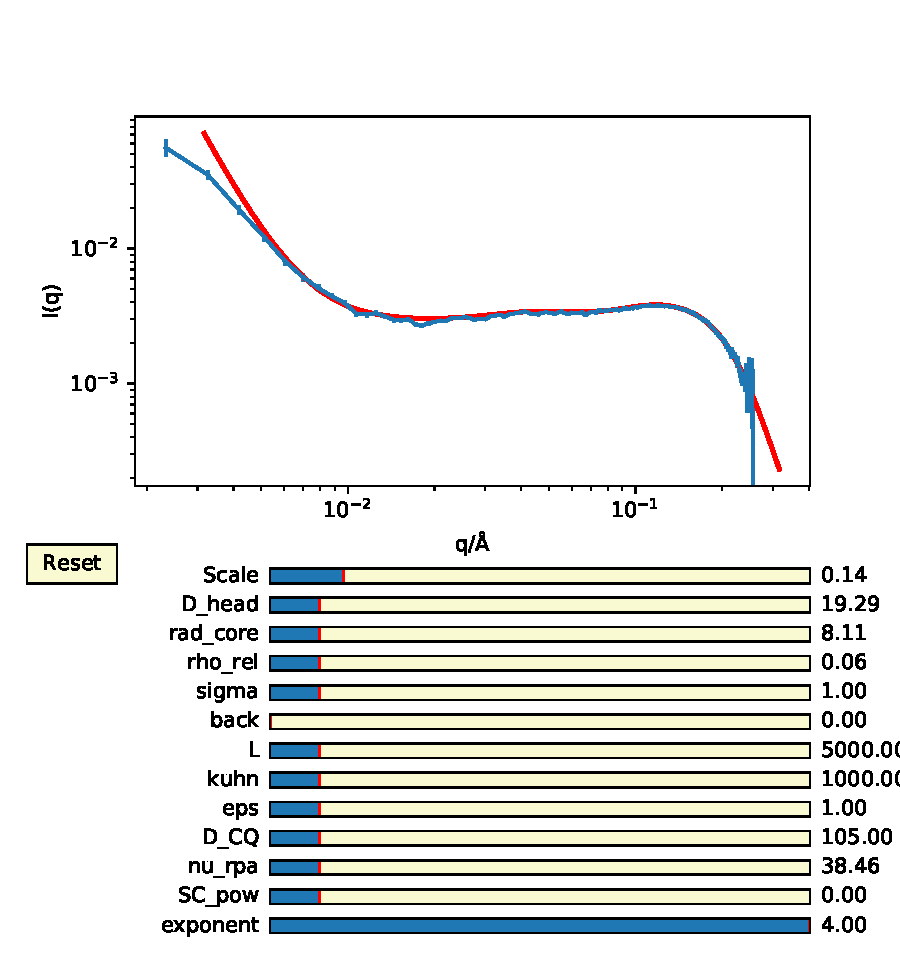
\includegraphics[width=0.7\textwidth]{imagens/saxs/Modelo_dado_SAXS_python}
	\caption{Dado real (azul) e modelo (vermelho) junto com os parâmetros de ajuste utilizados no modelo}
	\label{fig:saxs_modelo_dado_saxs_python}
\end{figure}

	Uma das motivações para realizar essa tarefa foi a grande dificuldade de nosso grupo utilizar SAXS para estudar micelas. Não há especialistas na região que conhecem modelagem de micelas gigantes. Além disso, escrever um modelo computacional baseando-se somente as equações matemáticas é uma tarefa muito difícil para quem não possui experiência. O modelo computacional, apesar de menos compacto em sua notação, é mais fácil de ser utilizado pois os passos são bastante detalhados, o que também facilita o entendimento de novos alunos. Além disso, examinando o código, é possível notar vários detalhes operacionais, como constantes de integração/normalização que não estão explicitamente presentes nas equações.
	
	As equações descritas no apêndice anterior foram traduzidas em uma série de funções e termos dentro dessas funções. Para ajudar no entendimento, há comentários no código que referenciam as equações à medida que elas são utilizadas. Note, porém, que a lógica utilizada para descrever um modelo matematicamente e computacionalmente são diferentes. Matematicamente, iniciei descrevendo o modelo de forma geral e depois descrevi as partes mais detalhadas, enquanto que, computacionalmente, essa ordem pode se inverter.
	
	Para facilitar o entendimento, a tabela \ref{tab:AP_corrs_blocos_equacoes} correlaciona as equações e os blocos de código onde aparecem.

\begin{table}[H]
	\IBGEtab{%
		\caption{Blocos de código e equações}
		\label{tab:AP_corrs_blocos_equacoes}
	}%
	{%
	\begin{tabular}{c c}
		\toprule
		          Bloco           & Equações                                                                                                       \\ \midrule
		   \ref{lst:WLM_geral}    & \ref{eqn:AP_Fcs}, \ref{eqn:AP_Fwc}, \ref{eqn:AP_Rc}, \ref{eqn:AP_Rs}, \ref{eqn:AP_saxs_MG_geral}, \ref{eqn:AP_Fsphere}  \\
		  \ref{lst:cadeia_KP_1}   & Tab. \ref{tab_ap:AiBi}                                                                                                  \\
		  \ref{lst:cadeia_KP_2}   & \ref{eqn:AP_Si}, \ref{eqn:AP_xi}, \ref{eqn:AP_Fwc}, \ref{eqn:AP_chi}                                                  \\
		  \ref{lst:cadeia_KP_3}   & \ref{eqn:AP_Ai}, \ref{eqn:AP_Bi}, \ref{eqn:AP_Gamma}, \ref{eqn:AP_Fwc}                                                \\
		\ref{lst:cadeia_KP_Debye} & \ref{eqn:AP_fdebye}, \ref{eqn:AP_w}, \ref{eqn:AP_FchainExV}                                                          \\
		 \ref{lst:cadeia_KP_SI}   & \ref{eqn:AP_Si}                                                                                                    \\ \bottomrule
	\end{tabular}%
}{}
\end{table}

As seguintes equações não aparecem no código:

\begin{table}[H]
	\IBGEtab{%
		\caption{Equações não descritas}
		\label{tab:AP_equacoes_n_descritas}
	}%
	{%
		\begin{tabular}{c p{10cm}}
			\toprule
			Equação   & Motivo  \\ \midrule
			\ref{eqn:AP_saxs_MG_superficial} & Melhor descrita pela Eq. \ref{eqn:AP_saxs_MG_geral} \\
			\ref{eqn:AP_saxs_PRISM} & O modelo PRISM, com uma aproximação, é calculado dentro da Eq. \ref{eqn:AP_saxs_MG_geral}  \\
			\ref{eqn:AP_Fwc_dois_casos} & Os dois casos são considerados simulaneamente durante os cálculos, então não é preciso realizar uma divisão explícita no código dos fatores \\
			\ref{eqn:AP_Rg2} & Devido aos parâmetros iniciais, o modelo não necessita calcular o raio de giro. \\
			\ref{eqn:AP_Frod}  & O modelo utiliza uma função para esfera ao invés de bastão no denominador, como uma aproximação \\ \bottomrule
		\end{tabular}%
	}{}
\end{table}

	\subsection{Código}

	\begin{listing}[H]
		\inputminted{python}{./python/cadeias_WLM_1.py}
		\caption{Cálculo das equações \ref{eqn:AP_saxs_MG_geral} e \ref{eqn:AP_Fsphere}}
		\label{lst:WLM_geral}
	\end{listing}
	
	\begin{listing}[H]
	\inputminted{python}{./python/cadeias_WLM_2.py}
	\caption{Aplicação da equação \ref{eqn:AP_saxs_MG_geral} para uma faixa de \q. É esta a função que deve ser importada em outros pacotes para fazer uso da modelagem}
	\label{lst:WLM_whole_q}
	\end{listing}
	
%	A parte mais complexa do modelo é justamente o modelo de Kratky-Porod com volume excluído para cadeias core-shell, e por isso merece uma subseção própria.

%	\subsection{Fator \(F_{KPchain_{ExV}}\)}
%	\label{sec:apendice_F_KPchain}
%	As equações da seção \ref{sec:equacoes_Fwc} relevantes ao cálculo do fator de cadeias com volume excluído então descritas nos códigos a seguir (listas \ref{lst:cadeia_KP_1}, \ref{lst:cadeia_KP_2}, \ref{lst:cadeia_KP_3}, \ref{lst:cadeia_KP_Debye}, \ref{lst:cadeia_KP_SI}).
%	
	\begin{listing}[H]
		\inputminted{python}{./python/cadeia_kratky_porod_inicial_1.py}
		\caption{Cálculo do fator de cadeias de Kratky-Porod com volume excluído (Parte 1/3)}
		\label{lst:cadeia_KP_1}
	\end{listing}

	\begin{listing}[H]
		\inputminted{python}{./python/cadeia_kratky_porod_inicial_2.py}
		\caption{Cálculo do fator de cadeias de Kratky-Porod com volume excluído (Parte 2/3)}
		\label{lst:cadeia_KP_2}
	\end{listing}

	\begin{listing}[H]
		\inputminted{python}{./python/cadeia_kratky_porod_inicial_3.py}
		\caption{Cálculo do fator de cadeias de Kratky-Porod com volume excluído (Parte 3/3)}
		\label{lst:cadeia_KP_3}
	\end{listing}

	\begin{listing}[H]
		\inputminted{python}{./python/cadeia_kratky_porod_inicial_4.py}
		\caption{Cálculo do fator de Debye}
		\label{lst:cadeia_KP_Debye}
	\end{listing}

	\begin{listing}[H]
		\inputminted{python}{./python/cadeia_kratky_porod_inicial_5.py}
		\caption{Cálculo numérico da integral cardinal}  % todo: encontrar um nome melhor
		\label{lst:cadeia_KP_SI}
	\end{listing}

\subsection{Uso do código}

Agora que todas as equações necessárias para descrever as micelas gigantes estão corretamente descritas programaticamente, é possível utilizar o modelo facilmente em outros projetos. Supondo que todas as funções criadas estejam num pacote chamado \texttt{SAXS\_FF}, é possível chamar a função e plotar um gráfico igual ao da Fig. \ref{fig:saxs_modelo_dado_saxs_python} com o seguinte código (\ref{lst:utilizando_modelo_WLM}), bastante simples:

\begin{listing}[H]
 	\inputminted{python}{./python/uso_modelo.py}
 	\caption{Exemplo de como utilizar o código de micelas gigantes para realizar um plot}  % todo: encontrar um nome melhor
 	\label{lst:utilizando_modelo_WLM}
\end{listing}
	
A partir deste ponto, é possível utilizar o código para realizar plotagens interativas, como também ajustes, utilizando métodos como \texttt{curve\_fit} do \texttt{scipy.optimize} ou, idealmente, o pacote \texttt{lmfit}.

\section{Descrição e uso do software de tratamento de curvas de fluxo}
\label{sec:apn_tratamento_CF}
Para o tratamento de dados de curva de fluxo, foi criado um programa que permite o usuário aplicar três modelos mais complexos e um modelo simplificado para a obtenção de valores de viscosidade no repouso. Todas as amostras, sem exceção, demonstraram ser pseudoplásticas, então não foram colocados mais modelos. A seguir, será mostrado os modelos utilizados e seções da lógica do programa, pois o código fonte inteiro é longo demais (aproximadamente 1000 linhas).

\subsection{Modelos de curvas de fluxo pseudoplásticas}
\label{sec:modelagem_curva_fluxo}
Foram implementados os modelos de \emph{Carreau-Yasuda} (Eq \ref{eqn:AP_CarreauYasuda}), \emph{Carreau} (Eq. \ref{eqn:AP_Carreau}), \emph{Cross} (Eq. \ref{eqn:AP_Cross}) e \emph{linear}, de maior para menor complexidade, respectivamente. Os modelos correlacionam a taxa de cisalhamento (\(\dot{\gamma}\), variável independente) à viscosidade (\(\eta\), variável dependente) utilizando alguns parâmetros.

\begin{equation}
	\eta = \eta_{\infty} + \frac{\eta_0 - \eta_{\infty}}{\left[  1 + \left(  \dfrac{\dot{\gamma}}{\dot{\gamma}_b}  \right)^{a}  \right]^{\frac{ \left(  n - 1  \right) }{a}}}
	\label{eqn:AP_CarreauYasuda}
\end{equation}

\begin{equation}
	\eta = \eta_{\infty} + \frac{\eta_0 - \eta_{\infty}}{\left[  1 + \left(  \dfrac{\dot{\gamma}}{\dot{\gamma}_b}  \right)^{2}  \right]^{\frac{n}{2}}}
	\label{eqn:AP_Carreau}
\end{equation}

\begin{equation}
	\eta = \eta_{\infty} + \frac{\eta_0 - \eta_{\infty}}{1 + \left(  \dfrac{\dot{\gamma}}{\dot{\gamma}_b}  \right)^{n}}
	\label{eqn:AP_Cross}
\end{equation}

O modelo linear considera somente valores de viscosidade em \(\dot{\gamma}\) próximos de zero, ou seja, \(\eta = \eta_0 + 0 \times \dot{\gamma}\).

Os parâmetros possuem os seguintes significados:

\begin{table}[H]
	\IBGEtab{%
          \caption{Parâmetros dos modelos de fluidos pseudoplásticos}
		  \label{tab:params_pseudoplasticos}
		}%
		{%
		\begin{tabular}{c c p{9cm}}
			\toprule
			   Parâmetro     & Unidade   & Significado                                                     \\ \midrule
			    \(\eta_0\)     & Pa.s      & Viscosidade no repouso*                                         \\
			\(\eta_{\infty}\)  & Pa.s      & Viscosidade no infinito                                         \\
			      \(n\)        & --        & Inclinação da região de decaimento de viscosidade               \\
			\(\dot{\gamma}_b\) & s\menosUm & \(\dot{\gamma}\) de início da região de decaimento de viscosidade \\ \midrule
			      \(a\)        & --        & Afeta tanto a inclinação quanto o ponto de inflexão             \\ \bottomrule
		\end{tabular}%
		}{}
\end{table}
% todo: encontrar a unidade de GPb
% todo: pensar em colocar os gráficos mostrando como esses parâmetros afetam as curvas
% todo: pensar um pouco mais sobre o Carreau-Yasuda e como que o a deve se comportar

A Fig. \ref{fig:reologia_modelos} exemplifica os modelos de Carreau e Cross e como os parâmetros afetam o formato das curvas. Note que a escala dos eixos é logarítmica. Vemos que, essencialmente, ambas as curvas possuem formatos muito semelhantes, com os parâmetros escolhidos. A escolha de um modelo depende da qualidade dos dados e do desejo do experimentalista. Observando-se como os modelos variam com os parâmetros, nota-se que a queda de viscosidade do modelo de Carreau é menos abrupta que no modelo de Cross e se assemelha mais aos dados estudados, então esse modelo foi mais utilizado.

\begin{figure}[H]
	\begin{subfigure}[t]{0.45\textwidth}
		\centering
		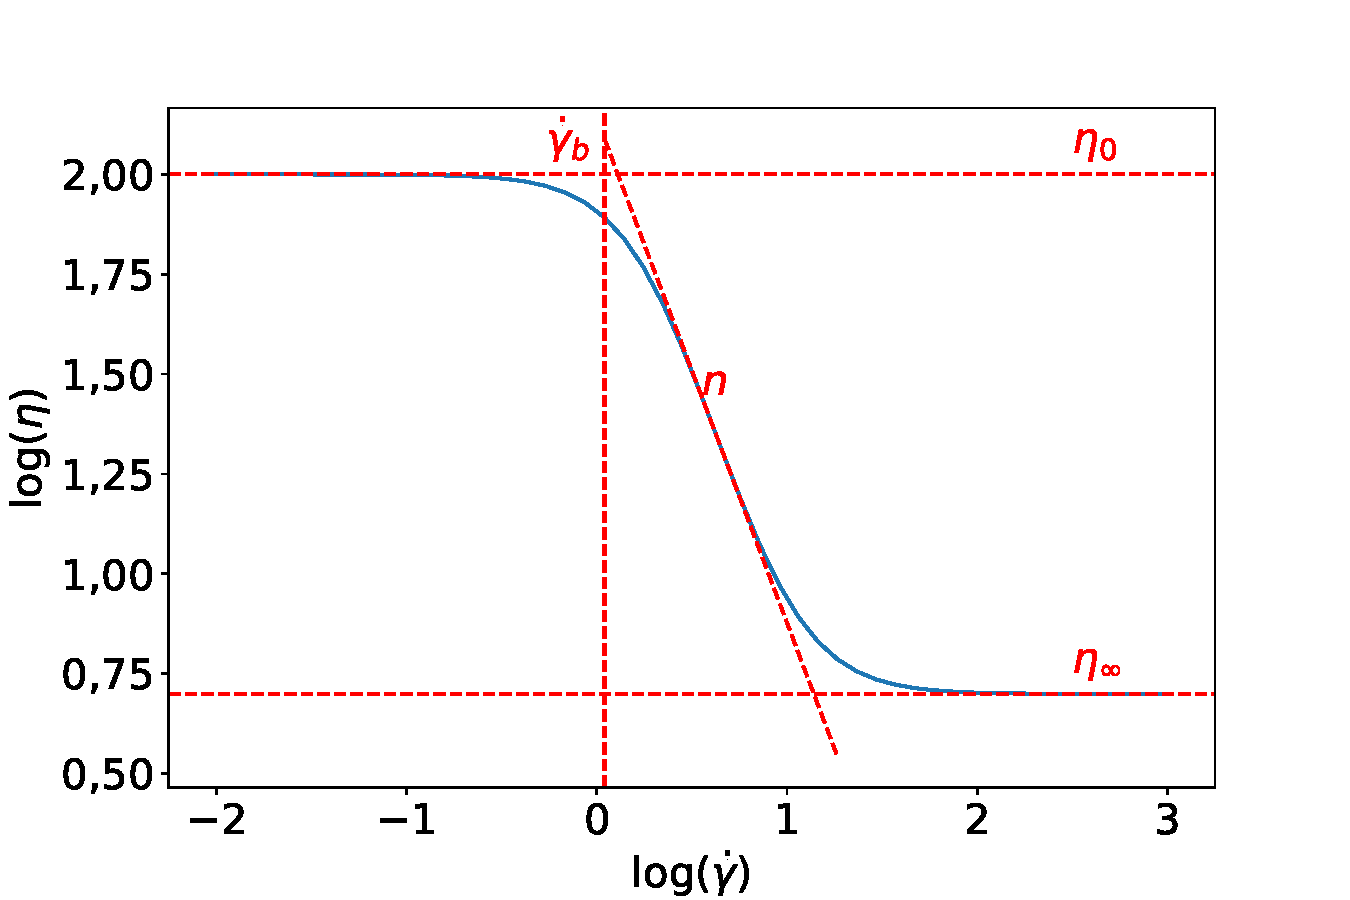
\includegraphics[width=\textwidth]{./imagens/reologia/Carreau}
		\caption{Modelo de Carreau}
		\label{fig:reologia_modelo_carreau}
	\end{subfigure} \qquad %
	\begin{subfigure}[t]{0.45\textwidth}
		\centering
		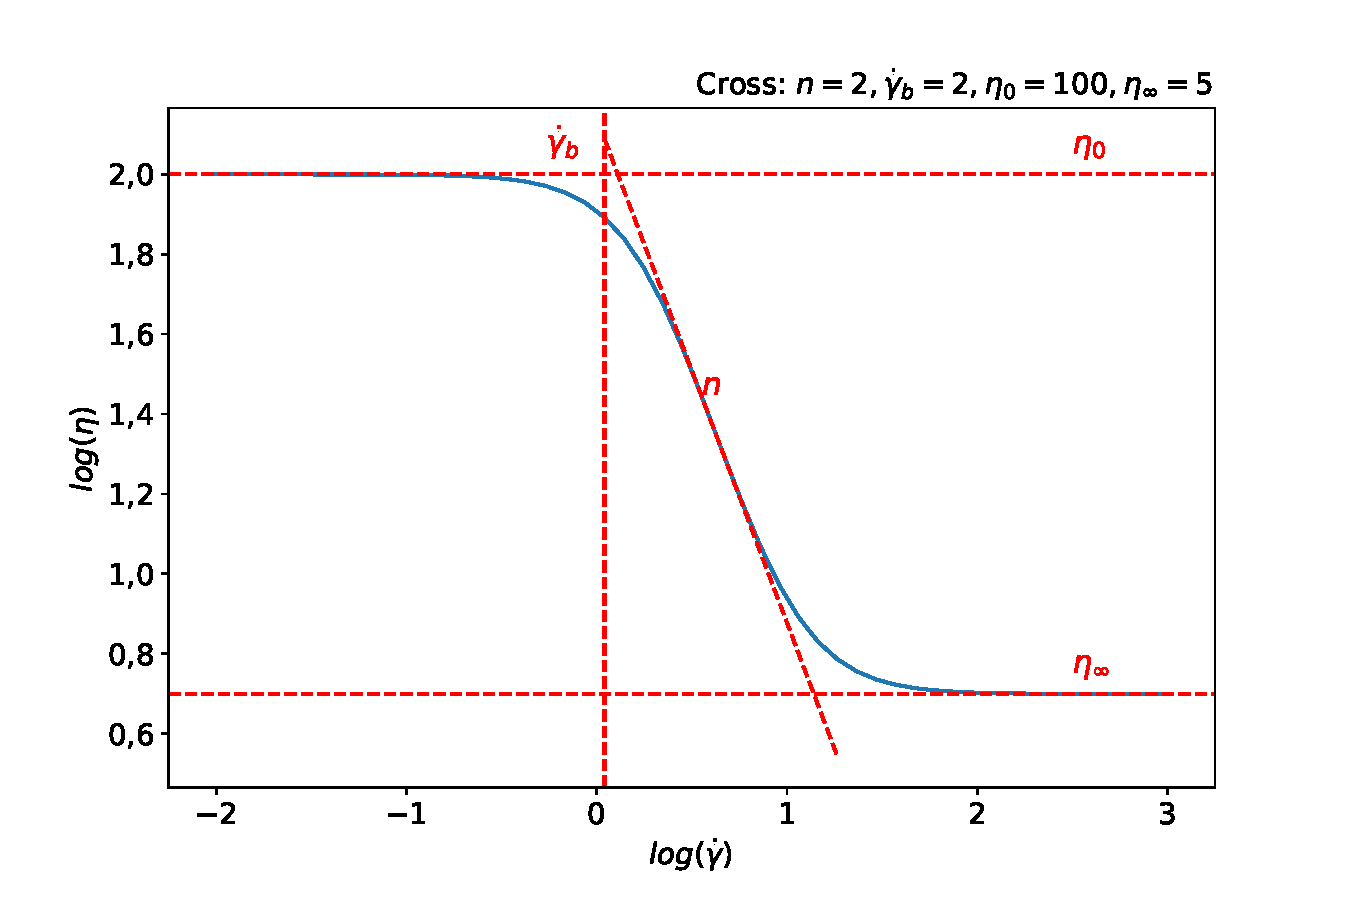
\includegraphics[width=\textwidth]{./imagens/reologia/Cross}
		\caption{Modelo de Cross}
		\label{fig:reologia_modelo_cross}
	\end{subfigure}
	\caption{Exemplos de curvas de fluxo descritas pelos modelos de Carreau e Cross, com os parâmetros utilizados.}
	\label{fig:reologia_modelos}
\end{figure}

De maior interesse para os estudos neste trabalho é a viscosidade no repouso, \(\eta_0\), e portanto esse é o foco do programa. Porém, o ajuste indiscriminado de um modelo a um dado experimental é problemático caso a qualidade do dado não seja boa, seja pela própria característica da amostra, ou pela sensibilidade do equipamento. Por exemplo, é frequente que apareçam artefatos de medida em baixos valores de \(\dot{\gamma}\), resultando ou num decréscimo ou acréscimo gradual de \(\eta\). Além disso, é possível que não seja observada a região descrita por \(\eta_{\infty}\), em altos valores de \(\dot{\gamma}\), o que atribui grande incerteza na determinação desse parâmetro. Dessa forma, é necessário que uma região das curvas seja escolhida para que o ajuste seja bem sucedido e informativo, o que representa a maior dificuldade nesse tipo de análise, devido à certa subjetividade no critério de escolha da região de ajuste.

Por essa razão, e outras, como velocidade de análise, foi escrito o método de ajuste. O método consiste em realizar ajustes sucessivos, entre um ponto inicial \(P_i\) até um ponto final \(P_f\), e depois comparar os resultados dos ajustes para escolher um deles. Podem ser comparados, por exemplo, os parâmetros \(R^2\), \(\chi^2\) ou \(\chi_{red}^2\). Escolhido o melhor ajuste, observando-se, por exemplo, a maior proximidade de \(R^2\) a 1 ou de \(\chi^2\) a 0, tomando cuidado para não escolher uma faixa muito estreita de pontos, os resultados são graficados, gravados num arquivo de texto e passa-se para o próximo dado experimental.

A listagem \ref{lst:exemplo_curva_de_fluxo} mostra duas seções do código completo do programa, uma mostrando o ciclo de ajuste utilizando o ajuste linear e \texttt{curve\_fit} e outro que realiza um ajuste não-linear utilizando o modelo de Carreau e \emph{lmfit}.

\begin{listing}[H]
	\inputminted{python}{./python/curva_de_fluxo.py}
	\caption{Seções do código mostrando o método de ajuste}  % todo: encontrar um nome melhor
	\label{lst:exemplo_curva_de_fluxo}
\end{listing}

Essas funções estão dentro de uma classe chamada \texttt{Fitter}. Para utilizar essa classe em outros códigos, é necessário inicializar uma instância da classe \texttt{Settings} e depois inicializar uma instância da classe \texttt{Fitter} utilizando as configurações da classe \texttt{Settings}. Caso não haja um arquivo \texttt{settings.dat} na pasta, um arquivo com valores padrão será criado. Após isso, é possível tanto editar o arquivo \texttt{settings.dat} quando utilizar as funções \texttt{print\_settings, edit\_settings} do objeto \texttt{Settings}. Ao criar um objeto \emph{Fitter}, por padrão os ajustes configurados já são realizados e os resultados são mostrados na tela. Caso se deseja criar um gráfico mostrando o resultado dos ajustes, pode-se chamar a função \texttt{plot\_error\_graphs()}. 

A listagem \ref{lst:exemplo_fitter} mostra como o programa pode ser utilizado por outros scripts, e o resultado do ajuste se encontra na Fig. \ref{fig:reologia_dado-exemplo}

\begin{listing}[H]
	\inputminted{python}{./python/uso_fitter.py}
	\caption{Exemplo de como utilizar a ferramenta de ajuste não linear}  % todo: encontrar um nome melhor
	\label{lst:exemplo_fitter}
\end{listing}

\begin{figure}[H]
	\centering
	\includegraphics[width=\textwidth]{imagens/reologia/Dado-exemplo}
	\caption{Figura resultante do ajuste não linear de Carreau e ajuste linear gerada pela função \texttt{plot\_error\_graphs()}. As barras de erro são oriundas da propagação de erro dos parâmetros e os números em vermelho indicam os pontos iniciais e finais considerados em cada ajuste.}
	\label{fig:reologia_dado-exemplo}
\end{figure}

Note que no dado utilizado, não há muitos problemas de desvio da curva, então os ajustes foram bem comportados. Os exemplos das figuras \ref{fig:reologia_dado-problemadescida} e \ref{fig:reologia_dado-problemasubida} mostram problemas reais na região de baixos valores de \(\dot{\gamma}\).

\begin{figure}
	\centering
	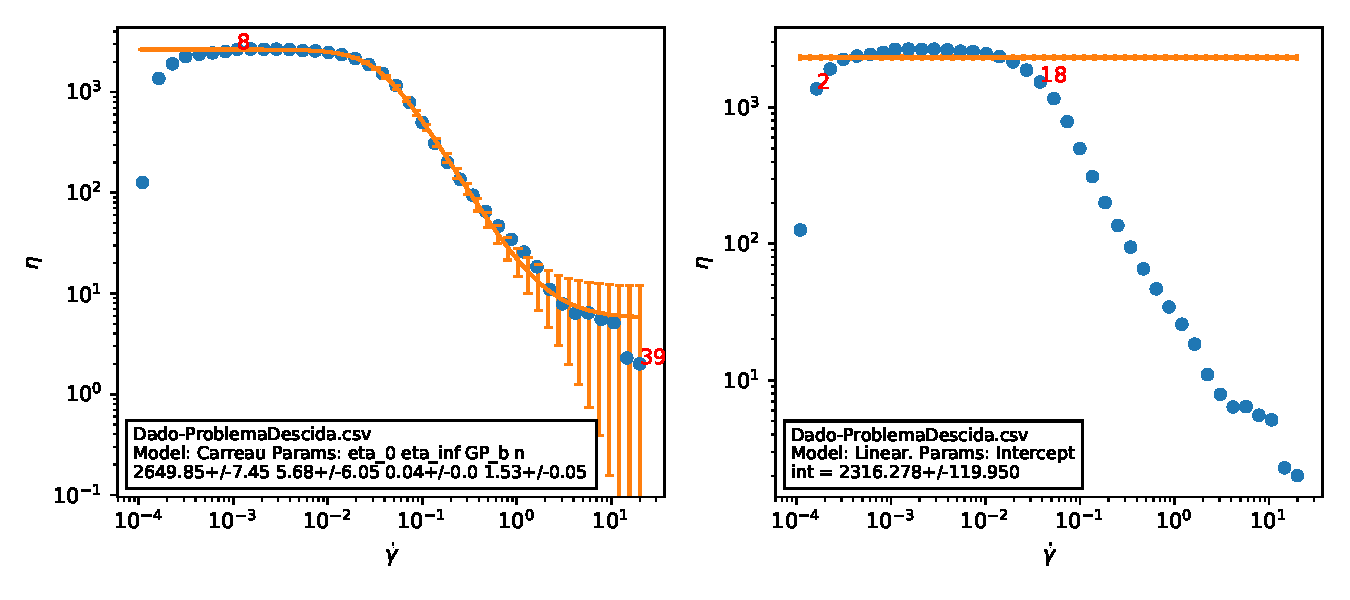
\includegraphics[width=\textwidth]{imagens/reologia/Dado-ProblemaDescida}
	\caption{Exemplo dos ajustes não-linear e linear de um dado real que possui uma queda nos valores de \(\eta\) em baixas \(\dot{\gamma}\)}
	\label{fig:reologia_dado-problemadescida}
\end{figure}

\begin{figure}
	\centering
	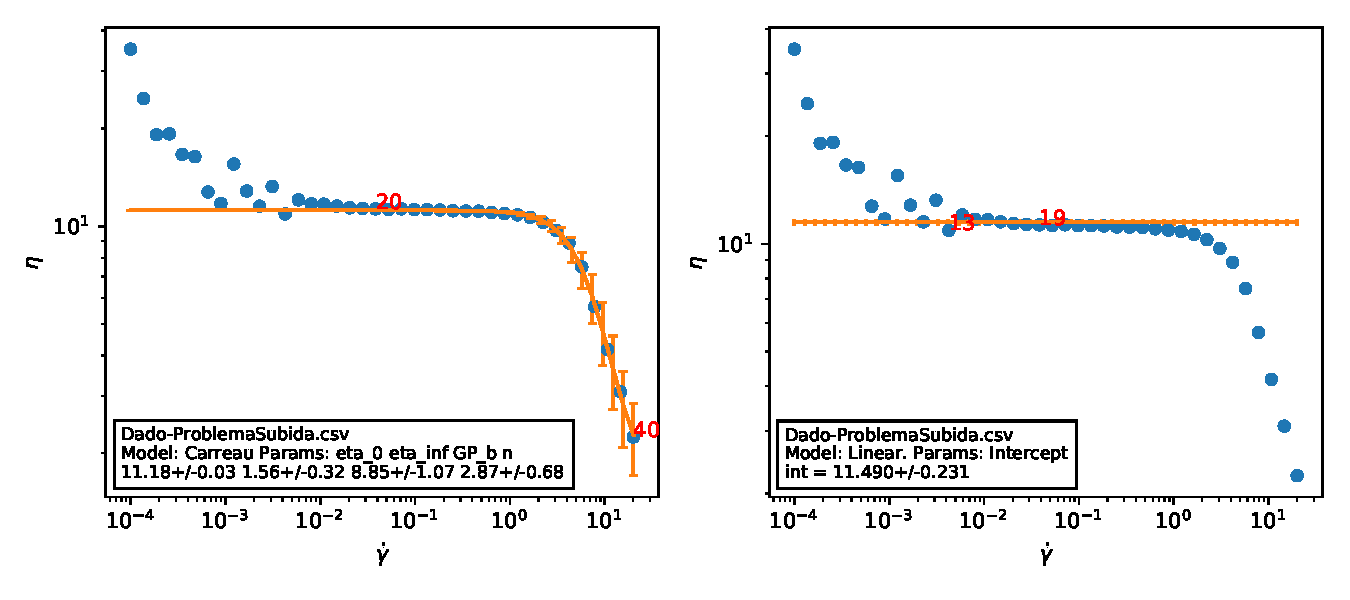
\includegraphics[width=\textwidth]{imagens/reologia/Dado-ProblemaSubida}
	\caption{Exemplo dos ajustes não-linear e linear de um dado real que possui um aumento nos valores de \(\eta\) em baixas \(\dot{\gamma}\)}
	\label{fig:reologia_dado-problemasubida}
\end{figure}

O tempo de execução e de plotagem para cada experimento está na faixa de um segundo, o que é muito mais rápido do que realizar o ajuste manualmente em uma ferramenta como o Origin ou Excel, então é algo ideal para o tratamento de um grande volume de dados.

\section{Método de ajuste para reologia oscilatória de muco}

Durante a execução do projeto de doutorado, foi estabelecida uma parceria com uma aluna de doutorado da Faculdade de Ciências Médicas na Unicamp, Carla Cristina S. Gomez, para a análise de amostras de muco de pacientes com fibrose cística. Foram realizadas medidas de curva de fluxo, analisadas pelo método descrito na seção \ref{sec:modelagem_curva_fluxo}. Além disso, foi necessário realizar uma análise das curvas de varredura de frequência para obter informações relevantes.

Plotando-se todos os dados obtidos, observou-se que G' estava sempre acima de G'' e, na escala logarítmica, as duas curvas eram praticamente paralelas e ligeiramente inclinadas positivamente. Em alguns casos, a inclinação aumentava em frequências maiores e, frequentemente, havia uma oscilação de G' e G'' sem significado físico nessa região. A taxa de aumento era consistente com uma exponencial. Visto isso, foi desenvolvido um script que realiza o seguinte:

\begin{enumerate}
	\item Obter a região de frequência confiável de G' e de G'' para o modelo linear e exponencial. Isso é feito realizando-se ajustes gradativos, do primeiro ponto até um ponto \emph{n}, armazenando os ajustes e depois escolhendo o ajuste com maior número de pontos onde \(R^2 > 0{,}9\). Caso não exista ajuste seguindo esse critério, escolhe-se um novo critério com \(R^2 > 0,85\). Caso não exista ajuste que obedeça isso mesmo assim, é escolhido o ajuste com o maior número de pontos. 
	\item Os parâmetros dos ajustes que passaram pelo filtro de \(R^2\) são gravados em um arquivo \texttt{csv}. Além disso, são gravados a média dos valores de G' e G'' da região linear, o desvio dessa média, o valor de \(R^2\), os índices dos pontos utilizados para o ajuste e o valor de G' e G'' em 0,6813Hz. Esses parâmetros foram escolhidos com base em alguns artigos da literatura. % todo: ref?
\end{enumerate}

Cerca de 500 dados experimentais únicos são tratados e plotados em cerca de 3 minutos, mostrando novamente o ganho enorme de eficiência com métodos computacionais. Após análise estatística, observou-se uma variação significativa em um dos conjuntos de dados. Porém devido à enorme variabilidade das amostras, houve pouca relevância estatística no resto do conjunto de dados. Contudo, os pacientes revelaram uma melhora física após o tratamento estabelecido, mostrando que de fato o tratamento foi eficiente. Mais informações sobre esse projeto podem ser encontrados na tese da aluna. O código fonte da parte de tratamento de dados está nas listagens \ref{lst:extracao_muco1} -- \ref{lst:extracao_muco6}. % todo: colocar uma referência pra tese dela.

\begin{listing}[H]
	\inputminted{python}{./python/extracao_muco1.py}
	\caption{Código fonte para a extração de informações de reologia oscilatória de muco (1/6)} 
	\label{lst:extracao_muco1}
\end{listing}

\begin{listing}[H]
	\inputminted{python}{./python/extracao_muco2.py}
	\caption{Código fonte para a extração de informações de reologia oscilatória de muco (2/6)} 
	\label{lst:extracao_muco2}
\end{listing}

\begin{listing}[H]
	\inputminted{python}{./python/extracao_muco3.py}
	\caption{Código fonte para a extração de informações de reologia oscilatória de muco (3/6)} 
	\label{lst:extracao_muco3}
\end{listing}

\begin{listing}[H]
	\inputminted{python}{./python/extracao_muco4.py}
	\caption{Código fonte para a extração de informações de reologia oscilatória de muco (4/6)} 
	\label{lst:extracao_muco4}
\end{listing}

\begin{listing}[H]
	\inputminted{python}{./python/extracao_muco5.py}
	\caption{Código fonte para a extração de informações de reologia oscilatória de muco (5/6)}
	\label{lst:extracao_muco5}
\end{listing}

\begin{listing}[H]
	\inputminted{python}{./python/extracao_muco6.py}
	\caption{Código fonte para a extração de informações de reologia oscilatória de muco (6/6)} 
	\label{lst:extracao_muco6}
\end{listing}


\section{Manual de uso do programa SUPERSAXS}
\label{sec:manual_SUPERSAXS}
Foi desenvolvido um guia para utilizar o programa SUPERSAXS, disponibilizado para o grupo. Aqui se encontra uma versão ligeiramente adaptada do manual.

\begin{center}
	\Huge{Tutorial para uso do programa SUPERSAXS}
	
	\Large{Karl Jan Clinckspoor}
	
	\large{26/10/2017}
\end{center}

\textbf{Resumo}

O programa SUPERSAXS foi desenvolvido em FORTRAN77 por Jan Skov Pedersen e Cristiano Oliveira, na Universidade de Århus, Dinamarca, para o ajuste não linear com base no método dos mínimos quadrados. A operação do programa é totalmente baseada no teclado. Este documento visa guiar um novo usuário a como utilizar o programa e alertá-lo para todos os eventuais problemas que possam aparecer.


\subsection*{Descrição geral}

O fluxo de trabalho do aplicativo segue a seguinte ordem.

\begin{enumerate}
	\item Carregar dados
	\item Plotar dados
	\item Escolha do modelo
	\item Chutes iniciais dos parâmetros
	\item Ajuste da curva
	\item Salvar parâmetros finais
\end{enumerate}

Quando se possui uma grande quantidade de arquivos para serem tratados, pode-se utilizar um processo de \emph{batch}, criando-se uma lista de arquivos para serem tratados automaticamente. Note que os dados não podem ser significativamente diferentes uns dos outros, senão o algoritmo de ajuste não consegue chegar numa resposta final satisfatória.

O programa é rodado utilizando-se o prompt de comando, o PowerShell ou somente dando duplo-clique no programa. A diferença do último método para os demais é que a janela se fecha imediatamente após o programa terminar.

Uma nova janela de prompt de comando ou PowerShell pode ser aberta na pasta atual clicando-se com o botão direito no Explorer com a tecla Shift apertada.

\begin{figure}[t]
	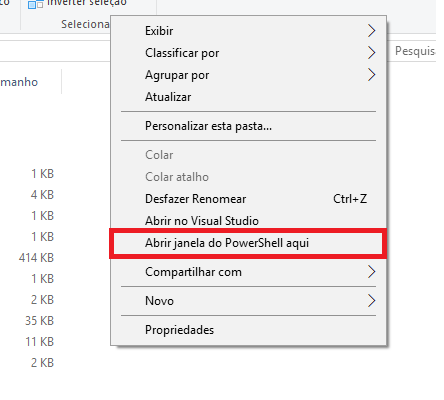
\includegraphics[scale=0.5]{./imagens/saxs/supersaxs_Powershell}
	\centering
	\caption{Como abrir uma janela do PowerShell no Windows 10}
	\centering
\end{figure}

Após isso, digite o nome do programa, geralmente \texttt{wlsq.exe} para iniciar o programa, e você será apresentado com a seguinte tela. Mas antes de realizar começar a fazer os ajustes, é necessário cuidar de outros detalhes.
\begin{samepage}
	\begin{verbatim}
	PS C:\Users\Karl\Desktop\SAXS\SAXS_Karl_back> .\wlsq_karl.exe
	*************************************************
	*                W L S Q S A X S                *
	*          LEAST SQUARES NONLINEAR FIT          *
	*               SUPERSAXS PROGRAMS              *
	*                                               *
	*EMPTY READY PROGRAM            crislpo 13/12/07*
	*************************************************
	
	FIT SINGLE FILE (0=def) OR LIST OF FILES (1) ?
	\end{verbatim}
\end{samepage}

\subsection{Carregamento de dados}

É necessário se atentar a estes três requesitos para os arquivos.

\begin{enumerate}
	\item Formatação
	\item Nome
	\item Localização
\end{enumerate}

\subsubsection{Formatação}

Os dados de SAXS devem obedecer a seguinte formatação:

\begin{linenumbers}
	\begin{verbatim}
	Comentário
	Comentário
	Número total de pontos
	q(nm ou Å) Int  Erro
	...     ...  ...
	\end{verbatim}
\end{linenumbers}
\resetlinenumber[1]

O valor de erro para as medidas não é necessário e o programa estima alguns valores. Um exemplo das primeiras linhas de um arquivo válido é:

\begin{linenumbers}
	\begin{verbatim}
	nothing special
	nothing special
	273
	0.0232465 0.021071 0.042898
	0.0325451 0.024961 0.013387
	0.0418437 0.012566 0.007131
	0.0511423 0.005719 0.004330
	0.0604409 0.003657 0.002916
	\end{verbatim}
\end{linenumbers}
\resetlinenumber[1]

\subsubsection{Nome}

O nome dos arquivos não pode conter espaços e deve ter no máximo 15 caracteres, incluindo a extensão. Dessa forma, \texttt{MG\_1.dat} é aceitável, mas \texttt{Micelas gigantes 1.dar} não é.

\subsubsection{Localização}
Os dados devem estar presentes na mesma pasta que o executável \texttt{wlsq.exe}. Além disso, não pode haver mais de 80 arquivos com a mesma extensão na pasta. Caso tenha que tratar mais de 80 arquivos, separe-os em subpastas e copie o executável para cada pasta.

\subsubsection{Arquivos adicionais}
Além dos arquivos com os dados de SAXS, os seguintes arquivos também devem estar presentes na pasta do executável.

\begin{itemize}
	\item \texttt{wgnuplot.exe}
	%\item \texttt{SAXS\{1\}N.DAT}
	\item \texttt{SAXS1N.DAT}
	\item \texttt{SAXS2N.DAT}
	\item \texttt{SAXS3N.DAT}
	\item \(\cdots\)
\end{itemize}

\texttt{wgnuplot.exe} é o programa utilizado para mostrar os dados e os ajustes. Os arquivos \texttt{SAXS\{numero\}N.DAT} contém parâmetros iniciais para os modelos \texttt{\{numero\}}. Por exemplo, se o modelo de micelas gigantes é o modelo número 2, \texttt{SAXS2N.DAT} irá conter os parâmetros iniciais para o modelo 2, neste caso, micelas gigantes.

\begin{verbatim}
0.15620869E+00 , 0,SCALE               
0.14915730E+02 , 0,D_HEAD              
0.10027541E+02 , 0,RAD_CORE            
0.12508109E+00 , 0,RHO_REL_OUT         
0.10000000E+01 , 1,sIGMA               
0.00000000E+00 , 1,BCK                 
0.50000000E+04 , 1,L_CONT              
0.10000000E+04 , 1,B_KUHN              
0.10000000E+01 , 1,EPS_XS              
0.92598854E+02 , 0,D_CQ                
0.40709053E+02 , 0,NU_RPA              
0.001,1,SC_POW
4,1,EXPONENT
\end{verbatim}

A falta desse tipo de arquivo gera um erro no programa na hora do início dos ajustes.

\subsection{Plotar dados}
Inicie o programa. Digite \texttt{0} e aperte enter para fazer o ajuste de um único arquivo. Em seguida, digite a extensão dos arquivos, geralmente \texttt{txt} ou \texttt{dat}. O programa irá listar todos os arquivos com aquela extensão na pasta.

\begin{verbatim}
Type desired file extension : dat

.dat FILES AVAILABLE:
1 100-60a.dat      21 PearlNl.dat
2 100-60o.dat      22 RESULT.DAT
3 A_100-60a.DAT    23 SalTB100.dat
4 A_34CB.DAT       24 SalTB55.dat
5 A_4CB.DAT        25 SalTB75.dat
6 A_92_30min.DAT   26 SAXS1N.DAT
7 A_final.DAT      27 SAXS2N.DAT
8 A_FT.DAT         28 SAXS2N_2.DAT
9 A_NaSal.DAT      29 SAXS3N.DAT
10 A_SalTB100.DAT   30 scanx.dat
11 A_SalTB55.DAT    31 SF.dat
12 A_SalTB75.DAT    32 test.dat
13 A_SF.DAT         33 TTAB.dat
14 A_TTAB.DAT
15 final.dat
16 FT.dat
17 initial.dat
18 LISTRES.DAT
19 OHCA6.dat
20 OHCA9.dat
FILENUMBER OF FILE TO BE FITTED :
\end{verbatim}

Digite o número do arquivo e aperte enter. Veja que o programa mostrou todos os arquivos, não só aqueles com dados válidos. Tentar carregar arquivos inválidos gera um erro no programa.

As seguintes frases irão aparecer, e os procedimentos a seguir são os mais comumente usados.

\begin{itemize}
	\item \texttt{INPUT SCALE FACTOR FOR THE FILE (1=def) :} não é necessário digitar nada, só apertar enter. Isso vale para a maior parte dos casos onde há um padrão, \emph{default}, \texttt{def}.
	\item \texttt{INPUT BACKGROUND FOR THE FILE (0=def) :} novamente, só apertar enter.
	\item \texttt{ADD EXTRA MC GENERATED NOISE (1/0=def)} só enter.
	\item \texttt{ESRF OR AARHUS DATA (1/2)}, digite 1 se os dados estiverem em \(nm^{-1}\) ou 2 se estiverem em \AA\(^{-1}\).
\end{itemize}

O programa irá então mostrar todo o conteúdo do arquivo e perguntar como deseja plotar os dados, começando com uma pergunta sobre o eixo Y e uma pergunta sobre o eixo X.

\begin{verbatim}
...      ...         ...           ...
316 0.266563714 1.09084343E-04 2.66976643
NO OF DATA POINTS  316
Which Function of Intensity;
Intensity[1], log(I)[2], log(q*I)[3], log(q*q*I)[4],1/I[5]
ln(I) [6], I*q**4[7] or I*q**2 [8]:
\end{verbatim}

Geralmente, seleciona-se \texttt{2}, ou seja, \(\log(I)\), e depois, para 
\begin{verbatim}Which Function of scattering vector;
q[1], q*q[2], log(q)[3] or q**4 [4] :\end{verbatim} seleciona-se \texttt{3}, para \(\log(q)\).

O programa irá então plotar o gráfico. A janela \emph{gnuplot pause} está com \emph{OK} selecionado então é possível fechá-la somente apertando enter novamente.

\begin{figure}[h]
	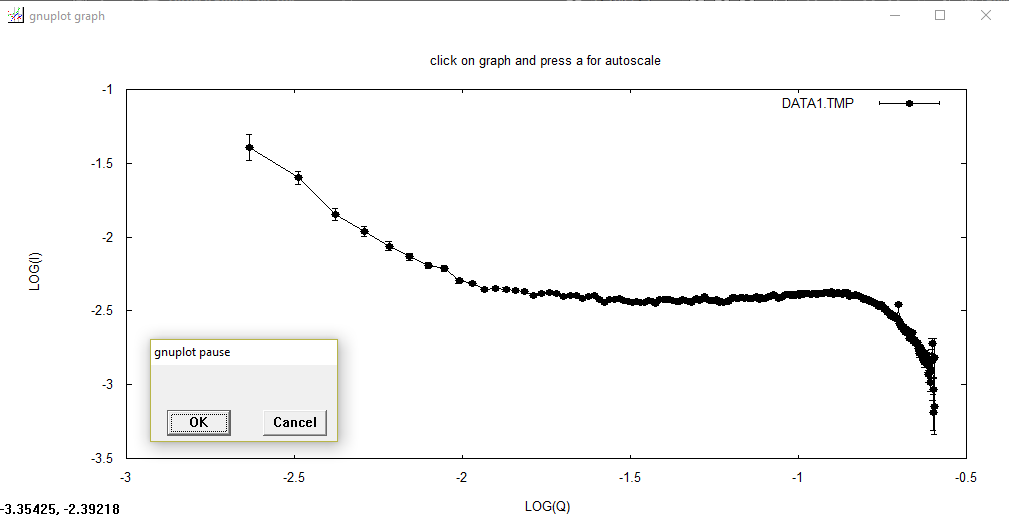
\includegraphics[scale=0.5]{./imagens/saxs/supersaxs_gnuplot}
	\centering
	\caption{Plot do dado na escala log-log}
	\centering
\end{figure}

\subsection{Escolha do modelo}

Aperte enter para:

\texttt{DO YOU WANT TO FIT (Y=def/N)}

e

\texttt{INCLUDE RESOLUTION FUNCTION (Y/N=def):}

Em seguida, o programa irá perguntar qual modelo se deseja ajustar:

\begin{verbatim}
CROSS SECTION
core-shell ELL MICS WITH HS S(Q)            (1)
Infinite LENGTH core-shell cylinder micelle (2)
3-ACIAL ELLIPSOID CORE-SHELL + S(Q)  HS     (3)
\end{verbatim}

Os modelos servem para:

\begin{enumerate}
	\item Micelas \emph{core-shell} elipsoidais (2-eixos) com fator estrutura \emph{hard spheres}.
	\item Micelas gigantes de Kratky-Porod (KP), core-shell, com interações intermoleculares modeladas pelo modelo PRISM.
	\item Micelas elipsoidais com 3 eixos e fator estrutura de \emph{hard spheres}
\end{enumerate}

Se há micelas esféricas, teste 1 primeiro, e depois 3, caso não consiga fazer o ajuste. Caso tenha micelas gigantes, selecione 2.

\subsection{Chutes iniciais}

A seguinte tela irá aparecer:

\begin{verbatim}
FILE OPENED
A( 1)=        0.15620869   IA( 1)= 0    SCALE
A( 2)=       14.91573050   IA( 2)= 0    D_HEAD
A( 3)=       10.02754120   IA( 3)= 0    RAD_CORE
A( 4)=        0.12508109   IA( 4)= 0    RHO_REL_OU
A( 5)=        1.00000000   IA( 5)= 1    sIGMA
A( 6)=    0.00000000E+00   IA( 6)= 1    BCK
A( 7)=     5000.00000000   IA( 7)= 1    L_CONT
A( 8)=     1000.00000000   IA( 8)= 1    B_KUHN
A( 9)=        1.00000000   IA( 9)= 1    EPS_XS
A(10)=       92.59885410   IA(10)= 0    D_CQ
A(11)=       40.70905300   IA(11)= 0    NU_RPA
A(12)=        0.00100000   IA(12)= 1    SC_POW
A(13)=        4.00000000   IA(13)= 1    EXPONENT
UNFIX SUBSET OF PARAMETERS    (-1)
FIX SUBSET OF PARAMETERS      (-2)
CHANGE MAX NO OF ITERATIONS   (99)
Change parameter no. (no change=0)
\end{verbatim}

\texttt{FILE OPENED} significa que o arquivo \texttt{SAXS2N.DAT} foi aberto com sucesso. Após isso, as linhas de \texttt{A( 1)} a \texttt{A(13)} possuem 4 colunas, que contém:

\begin{itemize}
	\item O número do parâmetro (1 a 13)
	\item O valor do parâmetro, em \AA.
	\item Se o parâmetro será fixado (1) ou está livre para variar (1)
	\item O nome do parâmetro.
\end{itemize}

Há 5 tipos de comandos que podem ser colocados nessa parte.

\begin{itemize}
	\item Número, de 1 a 13: Alterar o valor do chute e se o parâmetro será fitado ou não. A mensagem \texttt{Input A(I),IA(I)} irá aparecer. Escreva aqui o novo valor, uma vírgula, e 0 ou 1. Exemplo: \texttt{0.15,1}
	\item \texttt{-1}: Desfixar certos parâmetros. A seguinte mensagem irá aparecer: \texttt{INPUT I(MIN) I(MAX) FOR PARAMETERS TO BE UNFIXED}. Escreva A,B deixar variar todos os parâmetros entre A e B. Exemplo, escrever \texttt{3,7} irá desfixar os parâmetros entre 3 e 7, inclusivo. Se deseja fixar somente um parâmetros, escreva A,A (p.e. \texttt{1,1})
	\item \texttt{-2}: Fixar certos parâmetros. Mesma sintaxe que o anterior.
	\item \texttt{99}: Alterar o número de iterações do ajuste. O padrão é 10. Quando mais parâmetros, mais o fit demorará, mas melhor ele será.
	\item \texttt{0}: Nada será alterado, e o ajuste começará.
\end{itemize}

\subsection{Ajuste da Curva}
Ao escolher \texttt{0}, escolha o q mínimo e o q máximo para o ajuste. Esses valores deverão ser fornecidos na escala linear (não logarítmica). Geralmente \texttt{0.005} e \texttt{1} são o suficiente para pegar a faixa inteira. Isso pode ser usado para fitar somente algumas seções das curvas.

O programa começará a variar os parâmetros que foram deixados livres para minimizar o \(\chi^2\), a diferença entre os dados e o modelo. Em seguida, ele mostrará um plot com o modelo e os dados.

\begin{figure}[h]
	\centering
	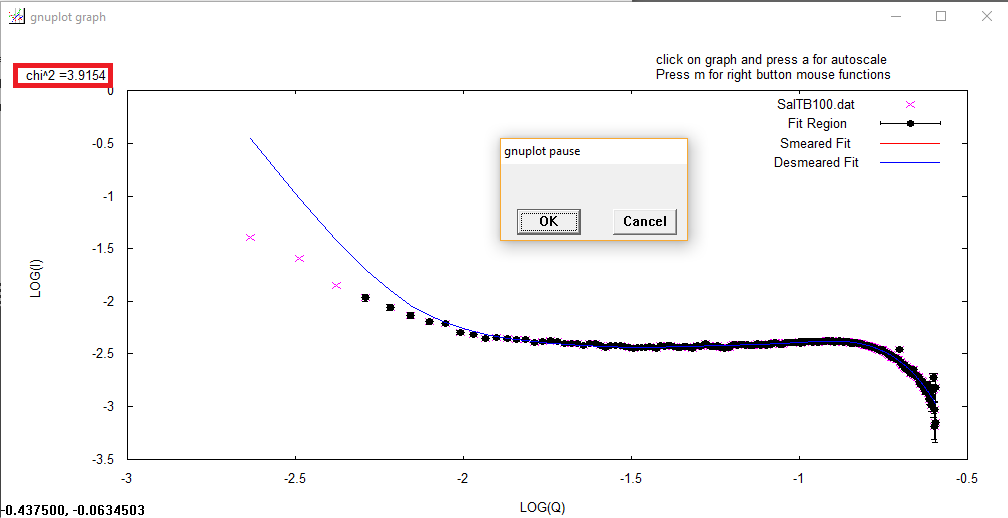
\includegraphics[scale=0.5]{./imagens/saxs/supersaxs_gnuplot_fit}
	\caption{Exemplo de um ajuste. Destacado está o \(\chi^2\) do ajuste.}
\end{figure}

E depois ele irá mostrar os parâmetros e os erros calculados de cada parâmetro.

\begin{verbatim}
*****PARAMETERS*****

INAL CHISQ= 0.402E+01   FINAL MSQRES= 0.392E+01

NO   START        FINAL        STD.ERR

1   0.1500E+00   0.1854E+00   0.6945E-02  SCALE
2   0.1492E+02   0.1381E+02   0.7423E+01  D_HEAD
3   0.1003E+02   0.7774E+01   0.1327E+01  RAD_CORE
4   0.1251E+00   0.1046E+00   0.9685E-01  RHO_REL_OUT
5   0.1000E+01   0.3933E+01   0.4168E+01  sIGMA
6   0.0000E+00   0.0000E+00   *FIXED      BCK
7   0.5000E+04   0.5000E+04   *FIXED      L_CONT
8   0.1000E+04   0.1000E+04   *FIXED      B_KUHN
9   0.1000E+01   0.1000E+01   *FIXED      EPS_XS
10   0.9260E+02   0.8345E+02   0.2666E+01  D_CQ
11   0.4071E+02   0.2835E+02   0.1814E+01  NU_RPA
12   0.1000E-02   0.1000E-02   *FIXED      SC_POW
13   0.4000E+01   0.4000E+01   *FIXED      EXPONENT
2.32465006E-03 325.344025 324.916748 325.344025 324.916748
2.32465006E-03 325.344025 324.916748 325.344025 324.916748
GIVE RETURN TO CONTINUE OR S=STORE
\end{verbatim}

Você tem duas escolhas, dar enter ou escrever \texttt{S}. Store armazena os parâmetros no arquivo \texttt{RESULT.DAT}, se você estiver satisfeito com os parâmetros.

Depois disso ele mostrará alguns parâmetros do ajuste e perguntar se você deseja fazer um novo fit. É necessário você escolher \texttt{Y} ou \texttt{N}. Aí você escolhe entre ajustar um novo conjunto de dados ou tentar ajustar esse dado novamente (\textit{default}). Aí o processo se repete.

\subsection{Resultados}

Neste exemplo, eu liberei o SC\_POW, fiz o ajuste novamente e salvei os parâmetros. Veja o ajuste.

\begin{figure}
	\centering
	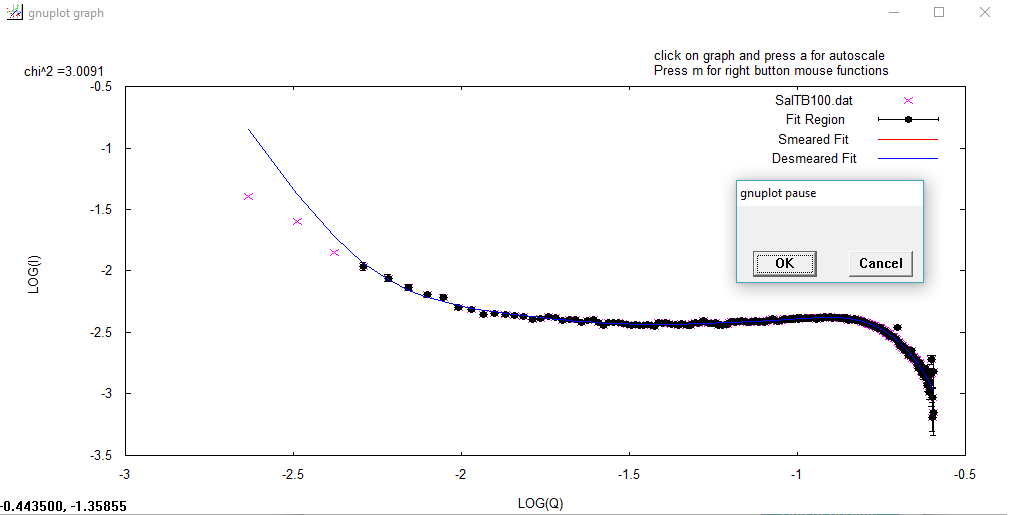
\includegraphics[scale=0.5]{./imagens/saxs/supersaxs_gnuplot_fit2}
	\centering
	\caption{Mesmo ajuste que o anterior, mas liberando o parâmetro \texttt{SC\_POW}}
\end{figure}

O arquivo \texttt{RESULT.DAT} contém as seguintes informações:

\begin{verbatim}
SalTB100.dat

FINAL CHISQ= 0.310E+01   FINAL MSQRES= 0.301E+01

NO   START        FINAL        STD.ERR

1   0.1854E+00   0.1850E+00   0.5645E-02  SCALE               
2   0.1381E+02   0.1358E+02   0.4355E+01  D_HEAD              
3   0.7774E+01   0.7320E+01   0.1081E+01  RAD_CORE            
4   0.1046E+00   0.1002E+00   0.5388E-01  RHO_REL_OUT         
5   0.3933E+01   0.4338E+01   0.2234E+01  sIGMA               
6   0.0000E+00   0.0000E+00   *FIXED      BCK                 
7   0.5000E+04   0.5000E+04   *FIXED      L_CONT              
8   0.1000E+04   0.1000E+04   *FIXED      B_KUHN              
9   0.1000E+01   0.1000E+01   *FIXED      EPS_XS              
10   0.8345E+02   0.8067E+02   0.2468E+01  D_CQ                
11   0.2835E+02   0.2531E+02   0.1475E+01  NU_RPA              
12   0.1000E-02   0.3958E-03   0.7098E-04  SC_POW              
13   0.4000E+01   0.4000E+01   *FIXED      EXPONENT            
\end{verbatim}

Esses valores podem então ser colocados numa planilha para serem plotados posteriormente.

Caso se coloque que não quer realizar um ajuste, o programa irá cair num estado pedindo sua escolha, caracterizado por \texttt{>} e o cursor piscante. Há 5 escolhas que podem ser feitas.

\begin{itemize}
	\item[FIT] Voltar e realizar um ajuste com a mesma função.
	\item[PLO] Plotar os dados e o ajuste.
	\item[FIL] Voltar ao início e escolher um novo arquivo e um novo modelo.
	\item[GRI] Faz ajustes pequenos de um número de parâmetros e mostra o valor de \(\chi^2\).
	\item[EXI] Sair do programa
\end{itemize}

\subsection{Análises em sequência}
\label{sec:script_saxs_sequencia}
Quando tiver muitos arquivos, você pode utiliar o modo de sequência, usando uma lista de arquivos. Essa lista deve ter o nome \texttt{INPUT.LIS} e deve conter o seguinte:

\begin{linenumbers}
	\begin{verbatim}
	Número de arquivos
	nome1.ext
	nome2.ext
	...
	\end{verbatim}
\end{linenumbers}
\resetlinenumber[1]

A lista tem um limite de arquivos, não muito grande. 30 arquivos é certamente factível, talvez 80 seja o máximo.

No programa, digite \texttt{1} no início para escolher o modo lista. A sequência de eventos é igual ao anterior, exceto na hora de escolher um novo arquivo. Quando você estiver satisfeito com a escolha dos parâmetros, coloque que deseja fazer um novo fit e depois que deseja fitar outro arquivo. Aí o programa irá fazer todos os arquivos, salvar no \texttt{RESULT.DAT}

Caso tenha muitos arquivos e deseje criar essa lista automaticamente, pode ser utilizado o script \texttt{converting\_files.py} para criar o script. Caso deseje converter o arquivo de resultados em algo um pouco mais fácil de ser importado para o excel, pode ser utilizado o script \texttt{converting\_results.py}, ambos disponíveis em \\https://github.com/KarlClinckspoor/SAXS\_treatment.

\section{Scripts menores para tratamento de dados}

Para acelerar o tratamento de dados, foram desenvolvidos alguns scripts para auxiliar na extração e conversão de arquivos, e para a obtenção de alguns valores. Esses scripts são, em sua maioria, bastante curtos e auto-explicativos, mas não necessariamente elegantes.

\subsection{Conversão de .dat do LNLS e Grenoble para arquivos compatíveis com o SUPERSAXS}

O programa SUPERSAXS necessita que existam duas linhas de comentário no cabeçalho do arquivo, seguido de uma linha com o número de pontos experimentais. Cada ponto experimental deve conter o valor de \q, em nm ou Å, intensidade e opcionalmente o erro (os valores de erro são estimados caso não estejam presentes). Além disso, o programa consegue analisar sequencialmente dados que possuem ajustes semelhantes, através de um arquivo \texttt{LIS}, que este script consegue criar também. Para executá-lo, basta rodar o comando \texttt{python converting\_files.py}. O código fonte se encontra nas listagens \ref{lst:conversao_supersaxs1} e \ref{lst:conversao_supersaxs2}.

\begin{listing}[H]
	\inputminted{python}{./python/converting_files1.py}
	\caption{Código fonte para o script de conversão de dados do ESRF e LNLS para um formato compatível com o programa SUPERSAXS (1/2)}  
	\label{lst:conversao_supersaxs1}
\end{listing}

\begin{listing}[H]
	\inputminted{python}{./python/converting_files2.py}
	\caption{Código fonte para o script de conversão de dados do ESRF e LNLS para um formato compatível com o programa SUPERSAXS (2/2)}  
	\label{lst:conversao_supersaxs2}
\end{listing}

\subsection{Conversão do arquivo RESULT.DAT para um arquivo .csv}

Os resultados dos ajustes do programa SUPERSAXS são gravados num arquivo chamado \texttt{RESULT.DAT}, sequencialmente. Porém, é trabalhoso importar esses dados para comparar os parâmetros de várias amostras, devido à sua formatação. Por esse motivo, foi criado um script que consegue converter esse arquivo em um arquivo \texttt{csv}.

\begin{listing}[H]
	\inputminted{python}{./python/converting_results.py}
	\caption{Código fonte para o script de conversão de resultados de ajuste do programa SUPERSAXS para csv}  
	\label{lst:conversao_resultados}
\end{listing}

\subsection{Conversão de .dat do LNLS para .pdh da Universidade de Graz}

O software \emph{SGI} desenvolvido pelo grupo do Prof. Otto Glatter da Universidade de Graz possui ferramentas que auxiliam na determinação de mesofases por meio da indexação de picos. O formato dos dados de SAXS obtidos no LNLS é incompatível com o formato requisitado pelo \emph{SGI}, então foi desenvolvido um pequeno script para realizar essa conversão. Esse script é simples o suficiente para poder ser transformado em executável com um programa como o pyinstaller.

O script encontra todos os arquivos \texttt{dat} da pasta onde o próprio se encontra e os transforma em \texttt{\_conv.dat}, que podem ser abertos diretamente pelo \emph{SGI}. O código fonte do script se encontra na listagem \ref{lst:LNLS_pdh}. Para utilizar este código, basta digitar no terminal \texttt{python LNLS\_dat\_to\_pdh.py} que a conversão será feita automaticamente.

\begin{listing}[H]
	\inputminted{python}{./python/LNLS_dat_to_pdh.py}
	\caption{Código fonte para o script the conversão de \texttt{dat} para arquivo similar ao \texttt{pdh} da Universidade de Graz}  % todo: encontrar um nome melhor
	\label{lst:LNLS_pdh}
\end{listing}

\end{apendicesenv}

\subsection{Desmembramento de arquivos exportados pelo software RheoWin}

Para a análise reológica completa de uma amostra, é necessário realizar uma sequência de experimentos no reômetro, que podem ser programados para ocorrerem sequencialmente. Os dados podem ser automaticamente exportados para um arquivo \texttt{txt} com todas as informações relevantes para uma análise, como os módulos G', G'', \(\eta\), etc. Não é possível, porém, exportar cada experimento separadamente, e a tarefa de separá-los manualmente é tediosa e passiva de erros. Por esses motivos, foi desenvolvido um script que consegue separar as seções dos arquivos \texttt{txt} em arquivos \texttt{csv}.

Por exemplo, o arquivo \texttt{Exp1.txt}, que possui reologia oscilatória de varredura de tensão, frequência e curvas de fluxo, é separado em três arquivos, \texttt{OT\_Exp1--0.csv}, \texttt{OF\_Exp1--0.csv} e \texttt{CF\_Exp1--0.csv}, respectivamente. O contador seguido do nome é necessário para diferenciar arquivos, caso haja colisão de nome. Para utilizar o script, somente é necessário colocá-lo na mesma pasta dos arquivos dos quais se deseja extrair dados e rodá-lo pelo console com \texttt{python Extracao\_dados.py}.

Como pré-requisitos, é necessário possuir o pacote \emph{pandas} do Python, que pode ser instalado pelo comando \emph{pip install pandas} e os arquivos devem ser exportados contendo, necessariamente, as seguintes colunas na seguinte ordem: número, taxa de cisalhamento, viscosidade, frequência, G', G'', temperatura, tensão.

O código fonte se encontra nas listagens \ref{lst:extracao_reologia1} e \ref{lst:extracao_reologia2}.

\begin{listing}[H]
	\inputminted{python}{./python/extracao_reologia1.py}
	\caption{Código fonte para o script de extração de dados de reologia fornecidos pelo software RheoWin (1/2)}  
	\label{lst:extracao_reologia1}
\end{listing}

\begin{listing}[H]
	\inputminted{python}{./python/extracao_reologia2.py}
	\caption{Código fonte para o script de extração de dados de reologia fornecidos pelo software RheoWin (2/2)} 
	\label{lst:extracao_reologia2}
\end{listing}

\subsection{Extração dos valores de largura de meia altura de curvas de DSC}
\label{sec:apendice_DSC}
Para determinar os valores das larguras de meia-altura, foi desenvolvido um pequeno script para limitar a subjetividade da determinação dessas quantidades. O script depende de um valor muito bom para a linha de base, que é tido como a mediana dos pontos de cada curva. Caso isso não seja obedecido, é necessário alterar o script para aceitar linhas de base diferentes. O código está nas listagens \ref{lst:meia_altura1} e \ref{lst:meia_altura2}.

\begin{listing}[H]
	\inputminted{python}{./python/meia_altura1.py}
	\caption{Código fonte para o script de obtenção dos valores de largura a meia altura de curvas de DSC (1/2)} 
	\label{lst:meia_altura1}
\end{listing}

\begin{listing}[H]
	\inputminted{python}{./python/meia_altura2.py}
	\caption{Código fonte para o script de obtenção dos valores de largura a meia altura de curvas de DSC (2/2)} 
	\label{lst:meia_altura2}
\end{listing}

%\begin{anexosenv}
%
%% Imprime uma página indicando o início dos anexos
%\partanexos
%
%% ---
%\chapter{Morbi ultrices rutrum lorem.}
%% ---
%\lipsum[30]
%
%% ---
%\chapter{Cras non urna sed feugiat cum sociis natoque penatibus et magnis dis
%parturient montes nascetur ridiculus mus}
%% ---
%
%\lipsum[31]
%
%% ---
%\chapter{Fusce facilisis lacinia dui}
%% ---
%
%\lipsum[32]
%
%\end{anexosenv}
